\documentclass[11pt,a4paper]{article}
\usepackage[utf8]{inputenc}
\usepackage[english]{babel}
\usepackage{amsmath,amsfonts,amssymb}
\usepackage{graphicx}
\usepackage{booktabs}
\usepackage{listings}
\usepackage{xcolor}
\usepackage{tikz}
\usepackage{algorithm}
\usepackage{algorithmic}
\usepackage{hyperref}
\usepackage{subcaption}
\usepackage{geometry}

\geometry{margin=1in}
\usetikzlibrary{shapes,arrows,positioning,fit,backgrounds,decorations.pathreplacing}

% Code configuration
\lstset{
    language=C++,
    basicstyle=\ttfamily\footnotesize,
    keywordstyle=\color{blue},
    commentstyle=\color{green!50!black},
    stringstyle=\color{red},
    breaklines=true,
    showstringspaces=false,
    frame=single,
    numbers=left,
    numberstyle=\tiny,
    tabsize=2
}

\lstdefinelanguage{Promela}{
    keywords={proctype,init,int,bool,byte,chan,mtype,inline,atomic,do,od,if,fi,goto,break,else,printf,run,never,ltl,true,false},
    keywordstyle=\color{blue}\bfseries,
    comment=[l]{//},
    commentstyle=\color{green!50!black},
    string=[b]",
    stringstyle=\color{red},
    basicstyle=\ttfamily\footnotesize,
    numbers=left,
    numberstyle=\tiny,
    breaklines=true,
    frame=single
}

\title{cpp-cache: A Formally Verified Concurrent Cache \\
with Single-Flight Coordination}
\author{Leandro Rabindranath Le\'{o}n \\
  \small SIMYL Research \\
  \small \url{https://github.com/lrleon/cpp-cache}}
\date{\today}

\begin{document}

\maketitle

\begin{abstract}
We present \textbf{cpp-cache}, a C++20 concurrent cache library whose
central design goal is not merely storing results but \emph{coordinating
concurrent access} to prevent redundant computation.  The library
implements the \emph{single-flight} pattern---at most one computation
per key at any time---combined with negative caching with independent
TTLs, LRU eviction with safety guarantees against use-after-free, and
explicit saturation signaling.

The concurrency protocol is formally verified using SPIN/Promela across
$\sim$3.5 million states, with 23 safety assertions and 10 LTL liveness
properties.  The formal model discovered a real bug---a missing refcount
check in the eviction path---that had survived code review and
conventional testing.

This paper describes the architecture, the concurrency model, the formal
verification approach and its results, the public API, and an honest
assessment of current limitations and tradeoffs.  The library is
open-source and has been validated in a production environment handling
100,000 requests per second.
\end{abstract}

\section{Introduction}

Cache systems are fundamental in modern software architectures.  However,
implementing a \emph{concurrent} cache presents challenges that go beyond
data storage.  The critical question is: \textbf{how should multiple
threads requesting the same key behave when the value is not yet
available?}

\subsection{The Core Problem: Thundering Herd}

Consider an expensive operation---a database query, an API call, a
complex calculation---that takes several seconds.  Without coordination,
multiple threads requesting the same key simultaneously each trigger
their own copy of the expensive operation:

\begin{lstlisting}[caption=Uncoordinated cache miss: N redundant computations]
Time T0:
  Thread 1: cache.get("key") -> MISS -> starts computation
  Thread 2: cache.get("key") -> MISS -> starts computation
  Thread 3: cache.get("key") -> MISS -> starts computation
  ...
  Thread N: cache.get("key") -> MISS -> starts computation

Result: N expensive operations for the same key.
\end{lstlisting}

This \emph{thundering herd} problem manifests in production as backend
overload, wasted CPU and memory, latency amplification, and cascade
failures when the backend cannot absorb the duplicate load.

\begin{figure}[htbp]
\centering
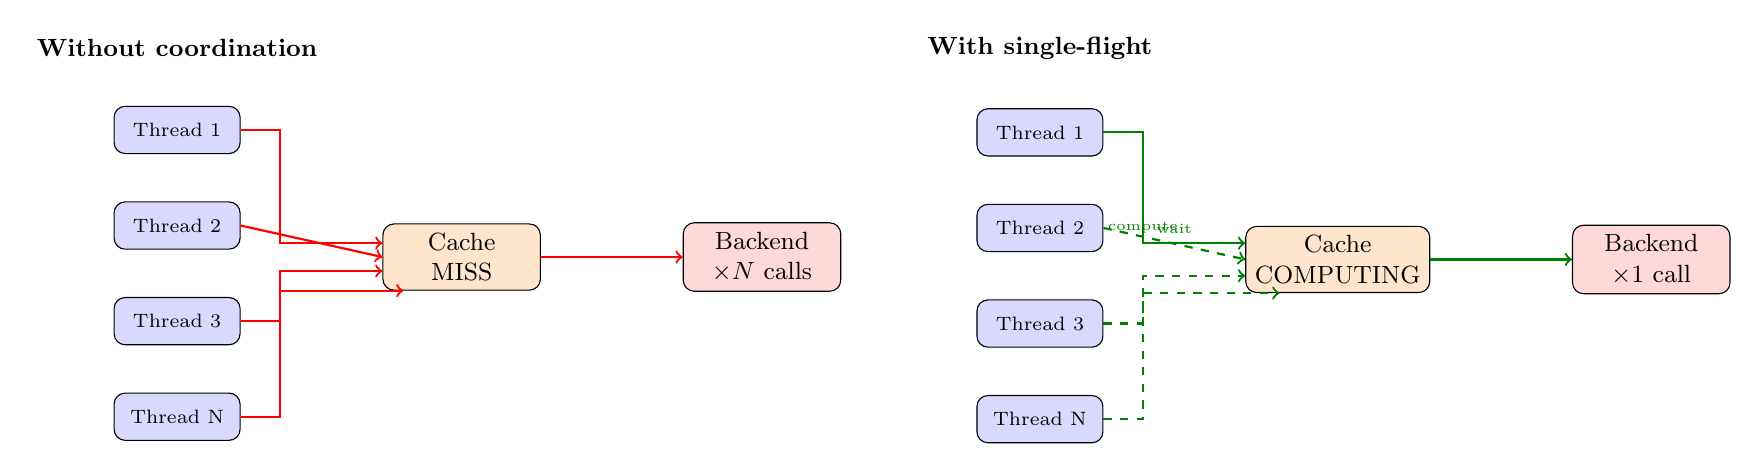
\begin{tikzpicture}[
    thread/.style={draw, rectangle, rounded corners, fill=blue!15,
                   minimum width=1.6cm, minimum height=0.6cm,
                   font=\scriptsize, align=center},
    cache/.style={draw, rectangle, rounded corners, fill=orange!20,
                  minimum width=2cm, minimum height=0.8cm,
                  font=\small, align=center},
    backend/.style={draw, rectangle, rounded corners, fill=red!15,
                    minimum width=2cm, minimum height=0.8cm,
                    font=\small, align=center},
    arrow/.style={->, thick},
    redarrow/.style={->, thick, red},
    greenarrow/.style={->, thick, green!50!black},
    dasharrow/.style={->, thick, dashed, green!50!black},
    node distance=0.6cm and 1.8cm
]

% Left side: thundering herd
\node[font=\bfseries\small] (title1) {Without coordination};
\node[thread, below=0.5cm of title1] (t1a) {Thread 1};
\node[thread, below=of t1a] (t2a) {Thread 2};
\node[thread, below=of t2a] (t3a) {Thread 3};
\node[thread, below=of t3a] (t4a) {Thread N};
\node[cache, right=of t2a, yshift=-0.4cm] (miss) {Cache\\MISS};
\node[backend, right=of miss] (be1) {Backend\\$\times N$ calls};

\draw[redarrow] (t1a.east) -- ++(0.5,0) |- (miss.170);
\draw[redarrow] (t2a.east) -- (miss.west);
\draw[redarrow] (t3a.east) -- ++(0.5,0) |- (miss.190);
\draw[redarrow] (t4a.east) -- ++(0.5,0) |- (miss.210);
\draw[redarrow] (miss) -- (be1);

% Right side: single-flight
\node[font=\bfseries\small, right=7.5cm of title1] (title2) {With single-flight};
\node[thread, below=0.5cm of title2] (t1b) {Thread 1};
\node[thread, below=of t1b] (t2b) {Thread 2};
\node[thread, below=of t2b] (t3b) {Thread 3};
\node[thread, below=of t3b] (t4b) {Thread N};
\node[cache, right=of t2b, yshift=-0.4cm] (coord) {Cache\\COMPUTING};
\node[backend, right=of coord] (be2) {Backend\\$\times 1$ call};

\draw[greenarrow] (t1b.east) -- ++(0.5,0) |- (coord.170)
  node[pos=0.5, above, font=\tiny] {compute};
\draw[dasharrow] (t2b.east) -- (coord.west)
  node[pos=0.5, above, font=\tiny] {wait};
\draw[dasharrow] (t3b.east) -- ++(0.5,0) |- (coord.190)
  node[pos=0.5, above, font=\tiny] {};
\draw[dasharrow] (t4b.east) -- ++(0.5,0) |- (coord.210);
\draw[greenarrow] (coord) -- (be2);

\end{tikzpicture}
\caption{Thundering herd (left): every thread triggers a backend call.
         Single-flight (right): one thread computes, others wait and
         share the result.  Backend receives one call instead of $N$.}
\label{fig:thundering-herd}
\end{figure}

\subsection{The Solution: A Cache as Coordination Mechanism}

A well-designed concurrent cache should enforce a simple invariant:

\begin{quote}
\emph{For any given key, at most one computation runs at a time.
Subsequent requests for the same key wait for the first computation
and share its result.}
\end{quote}

This is known as the \textbf{single-flight} pattern.  It is not a new
idea---Go's \texttt{singleflight} package, Google Guava's
\texttt{LoadingCache}, and Java's Caffeine all implement variants of
it.  What distinguishes cpp-cache is the combination of single-flight
with negative caching, safe lifetime management via reference counting,
and formal verification of the concurrency protocol.

\subsection{Scope of This Paper}

This paper describes \textbf{what the cpp-cache library provides}.
Deployment-specific concerns such as hash routing, circuit breakers, and
failover strategies are orthogonal to the library and are discussed
briefly in Appendix~\ref{sec:deployment} for context.

% ===================================================================
\section{Architecture}
\label{sec:architecture}
% ===================================================================

\subsection{Main Components}

The cache is built from three components:

\begin{enumerate}
\item \textbf{Hash table} (\texttt{LhashTableVtl<Key>}): Separate-chaining
      hash table with heap-allocated entries.  Provides $O(1)$ expected
      lookup and insertion.
\item \textbf{LRU list} (\texttt{Dlink}): Intrusive doubly-linked list
      for eviction ordering.  Each cache entry contains an embedded
      \texttt{Dlink} node.
\item \textbf{Cache entries} (\texttt{CacheEntry}): Heap-allocated
      objects that carry the key, value, state, TTL metadata, per-entry
      mutex, condition variable, and atomic reference count.
\end{enumerate}

\begin{figure}[htbp]
\centering
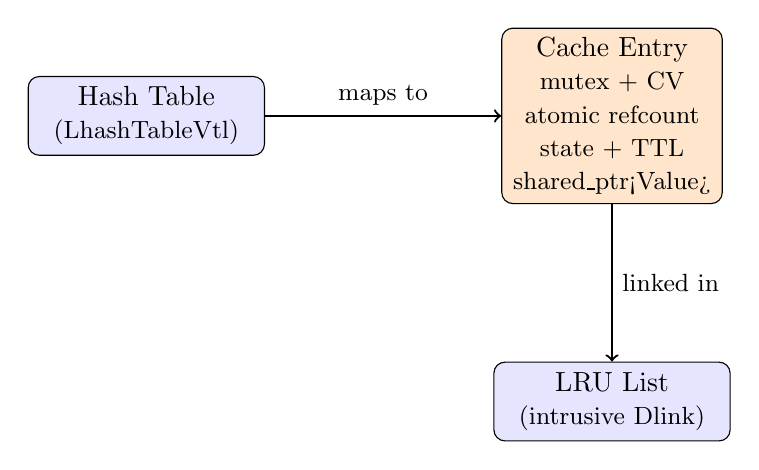
\begin{tikzpicture}[
    box/.style={draw, rectangle, rounded corners, fill=blue!10,
                minimum width=3cm, minimum height=1cm, align=center},
    entry/.style={draw, rectangle, rounded corners, fill=orange!20,
                  minimum width=2.8cm, minimum height=2.2cm, align=center},
    arrow/.style={->, thick},
    node distance=2cm and 3cm
]
\node[box] (hash) {Hash Table \\ \small (LhashTableVtl)};
\node[entry, right=of hash] (entry) {Cache Entry \\
  \small mutex + CV \\
  \small atomic refcount \\
  \small state + TTL \\
  \small shared\_ptr<Value>};
\node[box, below=of entry] (lru) {LRU List \\ \small (intrusive Dlink)};

\draw[arrow] (hash) -- (entry) node[midway,above] {\small maps to};
\draw[arrow] (entry) -- (lru) node[midway,right] {\small linked in};
\end{tikzpicture}
\caption{High-level architecture.  The hash table maps keys to
         heap-allocated entries.  Each entry is also linked into the
         LRU list via an intrusive \texttt{Dlink} node.}
\end{figure}

\subsection{Entry States}

Each cache entry maintains one of five states:

\begin{itemize}
\item \textbf{Empty}: Slot available; no key associated.
\item \textbf{Computing}: Miss solver is running.  The entry is
      \emph{not evictable} in this state.
\item \textbf{Ready}: Valid positive result cached (within TTL).
\item \textbf{Failed}: Computation failed or returned \texttt{nullptr};
      negative result cached (within negative TTL).
\item \textbf{Invalidated}: Logically removed; moved to LRU tail for
      priority eviction.
\end{itemize}

\begin{figure}[htbp]
\centering
\resizebox{\textwidth}{!}{
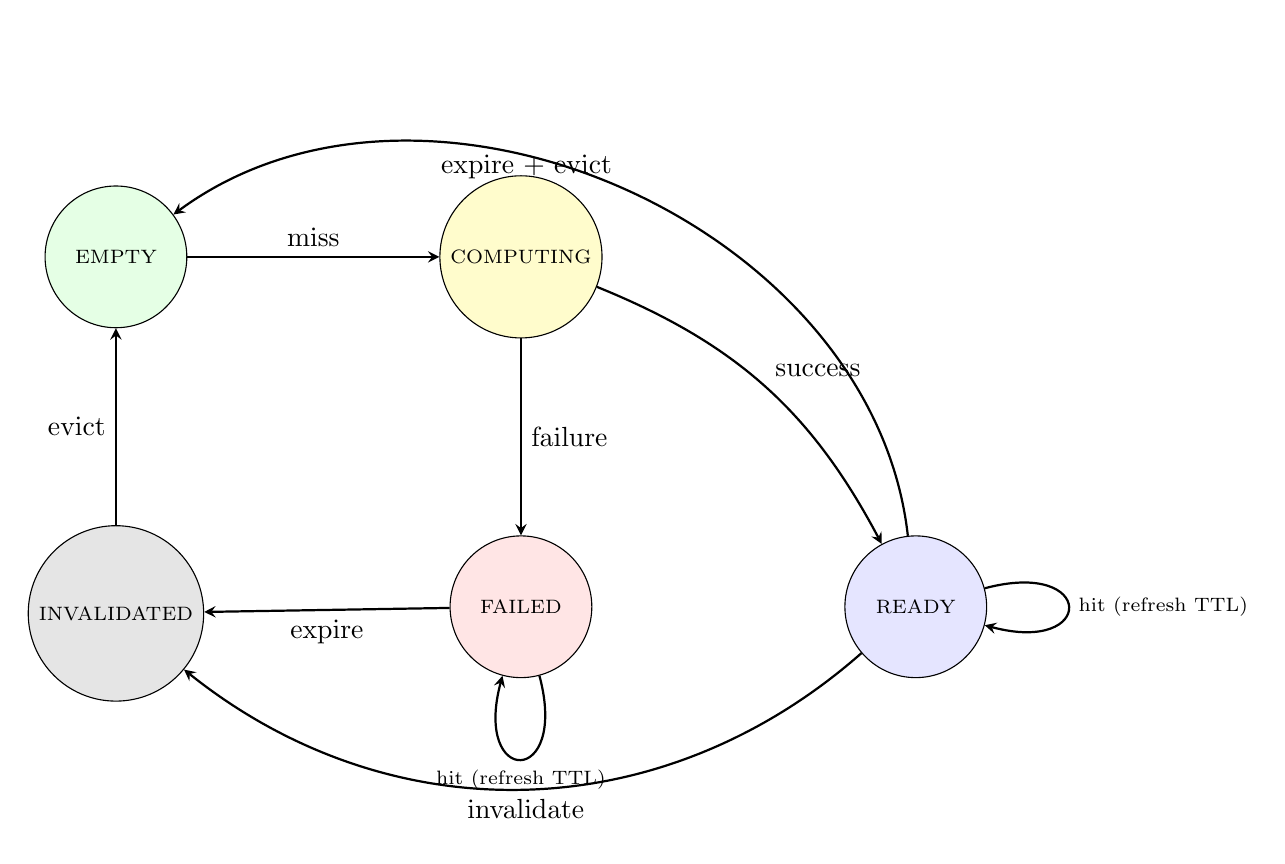
\begin{tikzpicture}[
    state/.style={circle, draw, minimum size=1.8cm, font=\scriptsize,
                  align=center},
    arrow/.style={->, thick, >=stealth},
    node distance=2.5cm and 3.2cm
]
\node[state, fill=green!10] (empty) {EMPTY};
\node[state, fill=yellow!20, right=of empty] (computing) {COMPUTING};
\node[state, fill=red!10, below=of computing] (failed) {FAILED};
\node[state, fill=blue!10, right=of failed] (ready) {READY};
\node[state, fill=gray!20, below=of empty] (invalidated) {INVALIDATED};

\draw[arrow] (empty) -- node[above] {miss} (computing);
\draw[arrow] (computing) -- node[right] {failure} (failed);
\draw[arrow] (computing) to[bend left=20] node[above right] {success} (ready);
\draw[arrow] (ready) to[bend left=40] node[below] {invalidate} (invalidated);
\draw[arrow] (failed) -- node[below] {expire} (invalidated);
\draw[arrow] (invalidated) -- node[left] {evict} (empty);
\draw[arrow] (ready) to[bend right=60] node[above left] {expire + evict} (empty);

% Self-loops for TTL refresh (sliding window)
\draw[arrow] (ready) to[loop right] node[right]
  {\scriptsize hit (refresh TTL)} (ready);
\draw[arrow] (failed) to[loop below] node[below]
  {\scriptsize hit (refresh TTL)} (failed);
\end{tikzpicture}
}
\caption{Complete state machine.  Self-loops on Ready and Failed
         represent sliding-window TTL refresh on every cache hit.}
\label{fig:state-machine}
\end{figure}

% ===================================================================
\section{Concurrency Model}
\label{sec:concurrency}
% ===================================================================

\subsection{Two-Level Locking}

The cache employs a hierarchical locking scheme:

\begin{enumerate}
\item A \textbf{global mutex} (\texttt{\_mtx}) protects the hash table
      structure and LRU list.  It is held only for brief structural
      operations: lookup, insert, evict, LRU reorder.  It is
      \emph{never held} during solver execution.
\item A \textbf{per-entry mutex + condition variable} implements
      single-flight coordination.  The first thread to trigger a miss
      marks the entry as \texttt{Computing}, releases the global lock,
      and runs the solver.  Subsequent threads for the same key block on
      the condition variable and share the result.
\end{enumerate}

This design ensures that different keys can be computed truly in
parallel.  The global lock serializes only the short structural
operations---hash lookup and LRU manipulation---while the potentially
expensive solver runs with no locks held.

\begin{figure}[htbp]
\centering
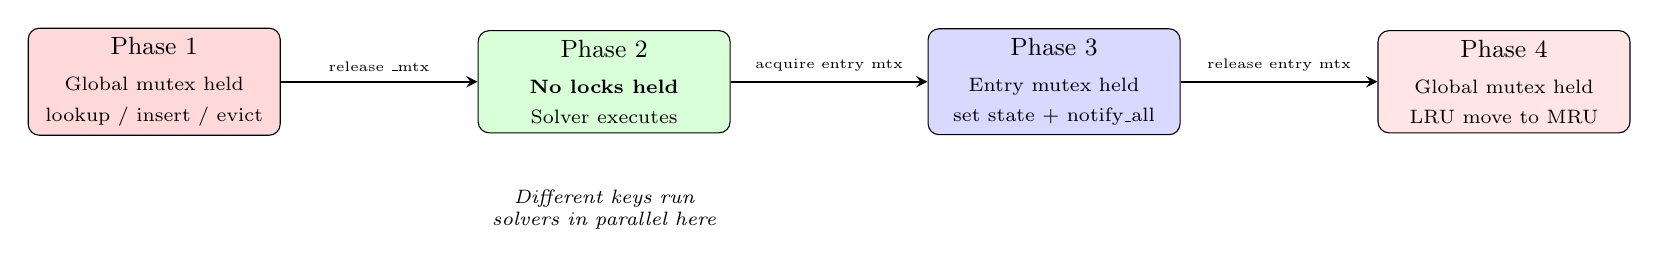
\begin{tikzpicture}[
    phase/.style={draw, rectangle, rounded corners, minimum width=3.2cm,
                  minimum height=1.2cm, align=center, font=\small},
    label/.style={font=\scriptsize, align=center},
    arrow/.style={->, thick, >=stealth},
    node distance=1.2cm and 2.5cm
]

% Phase 1
\node[phase, fill=red!15] (p1) {Phase 1\\[2pt]
  \scriptsize Global mutex held\\
  \scriptsize lookup / insert / evict};

% Phase 2
\node[phase, fill=green!15, right=of p1] (p2) {Phase 2\\[2pt]
  \scriptsize \textbf{No locks held}\\
  \scriptsize Solver executes};

% Phase 3
\node[phase, fill=blue!15, right=of p2] (p3) {Phase 3\\[2pt]
  \scriptsize Entry mutex held\\
  \scriptsize set state + notify\_all};

% Phase 4
\node[phase, fill=red!10, right=of p3] (p4) {Phase 4\\[2pt]
  \scriptsize Global mutex held\\
  \scriptsize LRU move to MRU};

\draw[arrow] (p1) -- (p2) node[midway, above, font=\tiny] {release \_mtx};
\draw[arrow] (p2) -- (p3) node[midway, above, font=\tiny] {acquire entry mtx};
\draw[arrow] (p3) -- (p4) node[midway, above, font=\tiny] {release entry mtx};

% Annotation
\node[below=0.6cm of p2, font=\scriptsize\itshape, align=center,
      text width=3.5cm] {Different keys run\\solvers in parallel here};

\end{tikzpicture}
\caption{Lock timeline for a cache miss.  The solver (Phase~2) runs with
         no locks held, enabling true parallelism across keys.  The
         global mutex is held only for brief structural operations.}
\label{fig:lock-phases}
\end{figure}

\begin{algorithm}[H]
\caption{Single-flight coordination for a cache miss}
\begin{algorithmic}[1]
\STATE \textbf{Thread 1} (first to arrive):
\STATE \quad Acquire global mutex
\STATE \quad Insert entry with state $\leftarrow$ \textsc{Computing}
\STATE \quad Release global mutex
\STATE \quad Execute miss solver (no locks held)
\STATE \quad Acquire entry mutex
\STATE \quad Set state $\leftarrow$ \textsc{Ready} or \textsc{Failed}
\STATE \quad \texttt{notify\_all()} on condition variable
\STATE \quad Release entry mutex
\STATE
\STATE \textbf{Threads 2, \ldots, N} (arrive during computation):
\STATE \quad Acquire global mutex
\STATE \quad Find entry with state = \textsc{Computing}
\STATE \quad Acquire refcount; release global mutex
\STATE \quad Acquire entry mutex
\STATE \quad \texttt{wait()} on condition variable
\STATE \quad Wake up; read the computed result
\STATE \quad Release entry mutex; release refcount
\end{algorithmic}
\end{algorithm}

\subsection{Lifetime Safety: Refcount + shared\_ptr}

A critical challenge in concurrent caches is preventing use-after-free
when an entry is evicted while another thread holds a pointer to it.
cpp-cache uses a two-tier lifetime model:

\begin{enumerate}
\item \textbf{Internal atomic refcount} on each \texttt{CacheEntry}.
      The table holds one reference; each thread operating on the entry
      acquires an additional reference via \texttt{acquire()}.  An RAII
      guard (\texttt{EntryGuard}) decrements the count on scope exit and
      deletes the entry if the count reaches zero.
\item \textbf{\texttt{shared\_ptr<Value>}} for the cached value itself.
      Callers receive a \texttt{shared\_ptr} that keeps the value alive
      independently of the cache's eviction decisions.
\end{enumerate}

This separation solves a real problem: without the refcount, evicting an
entry while another thread references it results in a dangling pointer.
The refcount check in \texttt{find\_evictable\_lru()}---entries are
evictable only if \texttt{refcount <= 1}---ensures that entries held by
active threads are never evicted.

\textbf{Notably, this invariant was discovered by the formal model}
(Section~\ref{sec:formal-verification}).

\begin{figure}[htbp]
\centering
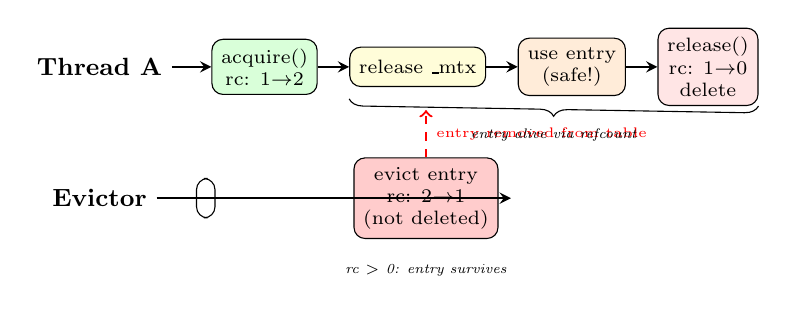
\begin{tikzpicture}[
    timeline/.style={draw, thick, ->, >=stealth},
    event/.style={draw, rectangle, rounded corners, font=\scriptsize,
                  minimum height=0.5cm, align=center},
    refbox/.style={draw, rectangle, rounded corners, fill=blue!10,
                   font=\scriptsize, minimum width=1cm, minimum height=0.5cm},
    note/.style={font=\tiny\itshape, align=center},
    node distance=0.3cm
]

% Thread A timeline
\node[font=\small\bfseries] (ta) {Thread A};
\node[event, fill=green!15, right=0.5cm of ta] (a1) {acquire()\\rc: 1$\to$2};
\node[event, fill=yellow!15, right=0.4cm of a1] (a2) {release \_mtx};
\node[event, fill=orange!15, right=0.4cm of a2] (a3) {use entry\\(safe!)};
\node[event, fill=red!10, right=0.4cm of a3] (a4) {release()\\rc: 1$\to$0\\delete};

\draw[timeline] (ta.east) -- (a1.west);
\draw[timeline] (a1.east) -- (a2.west);
\draw[timeline] (a2.east) -- (a3.west);
\draw[timeline] (a3.east) -- (a4.west);

% Eviction event
\node[font=\small\bfseries, below=1.2cm of ta] (tb) {Evictor};
\node[event, fill=white, right=0.5cm of tb] (b0) {};
\node[event, fill=red!20, right=2.5cm of tb] (b1) {evict entry\\rc: 2$\to$1\\(not deleted)};
\node[note, below=0.2cm of b1] {rc $>$ 0: entry survives};

\draw[timeline] (tb.east) -- ++(4.5,0);
\draw[->, thick, red, dashed] (b1.north) -- ++(0, 0.6)
  node[pos=0.5, right, font=\tiny] {entry removed from table};

% Brace showing entry alive
\draw[decorate, decoration={brace, amplitude=5pt, mirror}]
  (a2.south west) ++(0,-0.15) -- (a4.south east) ++(0,-0.15)
  node[midway, below=6pt, font=\tiny\itshape] {entry alive via refcount};

\end{tikzpicture}
\caption{Refcount lifetime safety.  Thread~A acquires a reference before
         releasing the global mutex.  Even if the evictor removes the
         entry from the table, the entry's memory remains valid until
         Thread~A's \texttt{EntryGuard} releases the last reference.}
\label{fig:refcount}
\end{figure}

\subsection{Saturation Handling}

When all entries are in \texttt{Computing} state or held by active
threads (\texttt{refcount > 1}), the cache cannot evict anything to make
room for a new key.  Rather than blocking indefinitely or silently
computing without caching (which would lose the single-flight guarantee),
\texttt{get\_or\_compute} returns a \texttt{CacheResult} with
\texttt{ResultOrigin::Saturated}.

This is an explicit signal that pushes the policy decision to the
caller:

\begin{lstlisting}[caption=Explicit saturation handling]
auto result = cache.get_or_compute(key);
if (result.is_saturated()) {
    // Caller decides: retry, return 503, compute directly, etc.
}
\end{lstlisting}

The cache tracks saturation events via \texttt{stats().saturations} for
monitoring.

% ===================================================================
\section{Public API}
\label{sec:api}
% ===================================================================

\subsection{Result Types}

All lookup operations return a \texttt{CacheResult<Value>} that
distinguishes the origin of the result:

\begin{itemize}
\item \textbf{HitPositive}: Value found in cache (valid, within TTL).
\item \textbf{HitNegative}: Cached failure found (within negative TTL).
\item \textbf{ComputedPositive}: Solver returned a value (newly computed).
\item \textbf{ComputedNegative}: Solver returned \texttt{nullptr} or
      threw an exception (newly failed).
\item \textbf{Saturated}: Cache full with no evictable entries.
\end{itemize}

This typed result enables callers to implement fine-grained telemetry
without guesswork about how the value was obtained.

\subsection{Graduated Lookup API}

The cache provides four lookup methods with different levels of blocking
and computation triggering:

\begin{table}[htbp]
\centering
\begin{tabular}{@{}llll@{}}
\toprule
Method & Blocks on Computing & Triggers Solver & TTL Refresh \\
\midrule
\texttt{get\_or\_compute(key)} & Yes (CV wait) & Yes & Yes \\
\texttt{find(key)} & Yes (CV wait) & No & Yes \\
\texttt{peek(key)} & No (try\_lock) & No & No \\
\texttt{has(key)} & No & No & No \\
\bottomrule
\end{tabular}
\caption{Comparison of lookup methods.  Note that \texttt{find()} blocks
         on \texttt{Computing} entries to maintain single-flight
         coherence---it is not a non-blocking call.  \texttt{peek()} is
         the truly non-blocking alternative.}
\label{tab:lookup-api}
\end{table}

\begin{lstlisting}[caption=Lookup API signatures]
// Primary: compute on miss, wait if Computing
CacheResult<Value> get_or_compute(const Key &key, Args... args);

// Read-only lookup: waits if Computing, never triggers solver
std::optional<CacheResult<Value>> find(const Key &key);

// Non-blocking: returns nullopt if entry busy or missing
std::optional<CacheResult<Value>> peek(const Key &key);

// Fast existence check (Ready or Failed, not expired)
bool has(const Key &key);
\end{lstlisting}

\subsection{Mutation Methods}

\begin{lstlisting}[caption=Mutation API]
// Marks entry as Invalidated, moves to LRU tail.
// Returns false if key not found or entry is Computing.
bool invalidate(const Key &key);

// Refreshes TTL and moves to MRU position.
// Returns false if expired, missing, or Computing.
bool touch(const Key &key);
\end{lstlisting}

Key design decisions:
\begin{itemize}
\item \texttt{invalidate()} refuses to invalidate \texttt{Computing}
      entries to avoid interrupting ongoing computations.
\item \texttt{touch()} implements sliding-window TTL refresh: each call
      extends the entry's lifetime by the full TTL duration.
\item There is no \texttt{remove()} method.  Only lazy invalidation is
      supported, which aligns with the reference Go implementation
      (\texttt{gateway\_cache}) and avoids ABBA deadlock risks from
      eager physical removal under concurrency.
\end{itemize}

\subsection{Variadic Miss Solver}

The miss solver supports arbitrary additional arguments via perfect
forwarding:

\begin{lstlisting}[caption=Variadic API with type-safe context propagation]
Cache<string, Data, equal_to<string>, DbConn&, int> cache(
    capacity, pos_ttl, neg_ttl,
    [](const string &key, DbConn &db, int txn_id) {
        return db.fetch(key, txn_id);
    }
);

auto result = cache.get_or_compute("key", db_conn, transaction_id);
\end{lstlisting}

This allows propagating opaque context (database connections, transaction
IDs, request metadata) to the solver without runtime overhead from type
erasure beyond the initial \texttt{std::function} wrapper.

\subsection{TTL Semantics: Sliding Window}

Both \texttt{get\_or\_compute()}, \texttt{find()}, and \texttt{touch()}
refresh the TTL on every access to a valid entry.  This implements a
\emph{sliding window} strategy: frequently accessed entries never expire
as long as accesses continue within the TTL interval.

This is a deliberate design choice aligned with the reference Go
implementation.  For use cases requiring \emph{fixed} TTL (absolute
expiration regardless of access frequency), the current API does not
offer a built-in option.  Users can approximate fixed TTL by avoiding
\texttt{find()} and \texttt{touch()} and using \texttt{peek()} for
read-only access that does not refresh TTL.

\subsection{Exception Handling in the Solver}

If the user-provided miss solver throws an exception, it is caught and
treated as a negative result (\texttt{ComputedNegative}).  The exception
itself is not propagated to the caller---all waiting threads receive the
negative result.

This design prevents one thread's exception from crashing waiting
threads, but it means the caller cannot distinguish ``solver returned
\texttt{nullptr}'' from ``solver threw an exception'' through the
\texttt{CacheResult} alone.  For debugging purposes, we recommend
logging exceptions inside the solver before rethrowing or returning
\texttt{nullptr}.

% ===================================================================
\section{Formal Verification}
\label{sec:formal-verification}
% ===================================================================

\subsection{Why Formal Verification?}

Concurrent systems fail in ways that conventional testing rarely
exposes.  Interleavings, rare races, and progress issues can survive
code review and even stress testing for years.  Formal model checking
explores \emph{all} reachable states exhaustively, providing guarantees
that no amount of testing can match for the properties being checked.

\subsection{Model Architecture}

The cache is modeled in Promela for verification with SPIN.  The model
faithfully captures:

\begin{itemize}
\item \textbf{Refcount semantics}: \texttt{slot\_rc[]} maps to
      \texttt{CacheEntry::\_refcount} and \texttt{EntryGuard} RAII.
\item \textbf{TTL aging}: \texttt{slot\_age[]} with a discrete threshold
      models sliding-window TTL refresh on hit.
\item \textbf{Three-phase locking}: Phase~1 (global lock: search/insert),
      Phase~2 (no lock: solver execution), Phase~3 (entry lock: state
      transition + CV notification).
\item \textbf{All five public API methods}: Separate processes model
      \texttt{get\_or\_compute}, \texttt{find}, \texttt{invalidate},
      \texttt{touch}, and \texttt{peek}.
\item \textbf{LRU eviction}: With the refcount guard
      (\texttt{slot\_rc[s] <= 1}).
\end{itemize}

\begin{table}[htbp]
\centering
\begin{tabular}{@{}llll@{}}
\toprule
Process & Instances & Type & Models \\
\midrule
\texttt{Requester} & 4 & One-shot & \texttt{get\_or\_compute()} \\
\texttt{FindRequester} & 2 & One-shot & \texttt{find()} \\
\texttt{Background} & 1 & Continuous & TTL aging + expiry \\
\texttt{Invalidator} & 1 & Continuous & \texttt{invalidate()} \\
\texttt{TouchRequester} & 1 & Continuous & \texttt{touch()} \\
\texttt{PeekRequester} & 1 & Continuous & \texttt{peek()} (try\_lock) \\
\bottomrule
\end{tabular}
\caption{10 concurrent processes in the verification model}
\end{table}

\subsection{Verified Properties}

\textbf{Safety (23+ assertions):} Verified exhaustively across $\sim$3.5
million states with zero errors.

\textbf{Liveness (10 LTL properties under weak fairness):}

\begin{lstlisting}[language=Promela, caption=Key LTL properties]
// All request threads eventually complete
ltl all_terminate {
  <> (request_done[0] && ... && request_done[5])
}

// No starvation: each thread eventually completes
ltl no_starvation_thread0 {
  [] (!request_done[0] -> <> request_done[0])
}

// Every requested key is eventually computed
ltl every_key_materializes {
  <> (ever_stored[0] && ever_stored[1] && ever_stored[2])
}
\end{lstlisting}

\subsection{Bug Found by the Model}
\label{sec:bug-found}

The formal model revealed a critical bug in the C++ implementation's
\texttt{find\_evictable\_lru()} function.  The original code checked
only the entry state before eviction but did not verify the reference
count:

\begin{lstlisting}[caption=Bug found by formal verification]
// BEFORE (bug): eviction possible with active holders
if (entry->state() != EntryState::Computing)
    return entry;  // UNSAFE: another thread may hold a reference

// AFTER (fix): aligned with Promela invariant slot_rc[s] <= 1
if (entry->state() != EntryState::Computing &&
    entry->_refcount.load(std::memory_order_acquire) <= 1)
    return entry;  // Safe: no external thread holds this entry
\end{lstlisting}

Without this check, a thread could evict an entry while another thread
was actively using it---a use-after-free that would manifest only under
specific timing conditions.  The Promela model's
\texttt{slot\_rc[s] <= 1} guard was already correct, exposing the
missing check in the C++ code.

\textbf{This is the strongest argument for formal verification in this
project}: it caught a real concurrency bug that survived code review and
conventional testing.

\subsection{Verification Results}

\begin{table}[htbp]
\centering
\begin{tabular}{@{}lrl@{}}
\toprule
Property & States & Result \\
\midrule
Safety (23+ assertions) & 3,500,000 & 0 errors \\
\texttt{all\_terminate} & depth 547 & 0 errors \\
\texttt{every\_key\_materializes} & depth 512 & 0 errors \\
\texttt{no\_starvation\_thread0..5} & depth 417--547 & 0 errors \\
\bottomrule
\end{tabular}
\caption{Exhaustive verification results (SPIN 6.5.2)}
\end{table}

% ===================================================================
\section{Test Suite}
\label{sec:tests}
% ===================================================================

The library is accompanied by a comprehensive test suite organized into
four tiers:

\begin{table}[htbp]
\centering
\begin{tabular}{@{}llr@{}}
\toprule
Category & Focus & Tests \\
\midrule
Unit tests & Basic functionality, negative caching, TTL, API & 29 \\
Hardened unit & Edge cases, solver behavior, LRU ordering, stats & 38 \\
Concurrency & Single-flight, parallel progress, races, stress & 11 \\
Hardened concurrency & Saturation, TOCTOU, TTL races, mixed ops & 19 \\
\midrule
\textbf{Total} & & \textbf{97} \\
\bottomrule
\end{tabular}
\caption{Test suite composition}
\end{table}

The CI pipeline runs these tests under multiple sanitizer configurations:

\begin{itemize}
\item \textbf{ASan + UBSan}: Detects memory errors and undefined behavior.
\item \textbf{TSan} (Clang): Detects data races.
\item \textbf{Valgrind}: Dedicated memory safety suite under concurrency.
\end{itemize}

% ===================================================================
\section{Comparison with Prior Art}
\label{sec:comparison}
% ===================================================================

\begin{table}[htbp]
\centering
\begin{tabular}{@{}lcccc@{}}
\toprule
Feature & cpp-cache & Go singleflight & Guava LoadingCache & Caffeine \\
\midrule
Single-flight per key & Yes & Yes & Yes & Yes \\
Negative caching & Yes (sep.\ TTL) & No & Yes (via Optional) & Yes \\
LRU eviction & Yes & N/A & Yes & Yes (W-TinyLFU) \\
Formal verification & \textbf{Yes (SPIN)} & No & No & No \\
Lock strategy & Global + per-entry & Per-key mutex & Segment locks & Lock-free \\
Self-contained & No (Aleph-w) & Yes & Yes & Yes \\
Benchmarks & No & N/A & Yes & Yes \\
\bottomrule
\end{tabular}
\caption{Comparison with established concurrent caches in other ecosystems}
\label{tab:comparison}
\end{table}

The formal verification is a genuine differentiator---none of the
compared alternatives provide exhaustive model checking of their
concurrency protocols.

% ===================================================================
\section{Known Limitations and Tradeoffs}
\label{sec:limitations}
% ===================================================================

We believe an honest assessment of limitations strengthens rather than
weakens a project's credibility.

\subsection{Global Mutex as Potential Bottleneck}

The global mutex serializes every structural operation.  While critical
sections are short (hash lookup + LRU manipulation), under extremely
high concurrency with thousands of threads and high miss rates, this
single lock could become a contention point.

High-performance alternatives use sharded/striped locks (e.g., Java's
\texttt{ConcurrentHashMap} with 16 segments) or lock-free hash tables.
The current design trades peak throughput for simplicity and
correctness---a reasonable choice when the solver is the real bottleneck,
as is typically the case.

\textbf{Planned mitigation}: Sharding into $N$ sub-caches, each with
its own mutex, table, and LRU list.  Key-to-shard mapping via
\texttt{hash(key) \% N} would provide linear scalability with cores
without changing the per-shard semantics.

\subsection{Dependency on Aleph-w}

The library depends on \texttt{Aleph-w}~\cite{alephw} for its hash
table (\texttt{LhashTableVtl}) and intrusive linked list
(\texttt{Dlink}).  This creates adoption friction:

\begin{itemize}
\item Users must clone Aleph-w as a sibling directory (CMake searches
      multiple candidate paths).
\item Aleph-w carries transitive dependencies (GSL, X11, MPFR) that
      are not needed by the cache itself.
\item The \texttt{LINKNAME\_TO\_TYPE} macro uses null pointer arithmetic
      that triggers UBSan, requiring \texttt{-fno-sanitize=null}.
\end{itemize}

We chose Aleph-w because its intrusive data structures provide better
cache locality and avoid extra allocations compared to
\texttt{std::unordered\_map} + \texttt{std::list}.  However, we
acknowledge this is the biggest barrier to adoption and plan to evaluate
a self-contained mode in the future.

\subsection{No Benchmarks in the Repository}

Despite production validation at 100K req/sec, the repository currently
lacks microbenchmarks.  Users cannot independently:

\begin{itemize}
\item Compare throughput against alternatives.
\item Measure global mutex contention under varying concurrency.
\item Profile hit/miss ratios at different key distributions.
\end{itemize}

Adding a benchmark suite (e.g., using Google Benchmark) with scenarios
like ``$N$ threads, $M$ keys, $X$\% miss rate'' is planned as near-term
work.

\subsection{Sliding TTL Only}

The TTL refresh on every hit (sliding window) means frequently accessed
entries may never expire.  The API does not currently offer a fixed-TTL
mode for data with absolute freshness requirements.

\subsection{Exception Information Lost}

When the solver throws, the exception is caught and treated as a
negative result.  The caller receives \texttt{ComputedNegative} with no
indication that an exception occurred versus the solver returning
\texttt{nullptr}.  Logging exceptions inside the solver is the
recommended workaround.

% ===================================================================
\section{Production Heritage}
\label{sec:production}
% ===================================================================

The design follows a pattern proven in \texttt{gateway\_cache}, a Go
implementation with 6 years of production use handling $\sim$100K
req/sec for sports fixture data.  cpp-cache is a C++20 reimplementation
that aligns its concurrency model with the Go reference while addressing
C++-specific challenges (manual lifetime management, absence of garbage
collection).

Key production metrics from the Go deployment:

\begin{table}[htbp]
\centering
\begin{tabular}{@{}lrl@{}}
\toprule
Metric & Value & Notes \\
\midrule
Throughput & 100,000 req/sec & Production load \\
p95 latency (hit) & $<$ 5ms & Cache hit path \\
Hit ratio & $>$ 95\% & Fixture data with temporal locality \\
\bottomrule
\end{tabular}
\caption{Production performance metrics from the Go reference implementation}
\end{table}

% ===================================================================
\section{Conclusions}
% ===================================================================

cpp-cache addresses a well-defined problem: coordinating concurrent
access to expensive-to-compute resources through a cache that enforces
single-flight behavior per key.  The combination of:

\begin{itemize}
\item A clean five-state machine with explicit transitions,
\item Two-level locking (global for structure, per-entry for coordination),
\item Refcount-based lifetime safety verified by formal model,
\item Negative caching with independent TTLs,
\item Explicit saturation signaling,
\item 97 tests across four tiers plus sanitizer validation,
\item And genuine formal verification that caught a real bug,
\end{itemize}

\noindent places it above the typical open-source C++ cache library in
terms of correctness confidence.

The main barriers to wider adoption are the Aleph-w dependency, the
absence of benchmarks, and the sliding-only TTL policy.  Addressing
these is planned as future work and would transform cpp-cache from a
solid internal tool into a compelling general-purpose offering.

% ===================================================================
\section{Future Work}
% ===================================================================

\begin{enumerate}
\item \textbf{Benchmarks}: Google Benchmark suite with configurable
      thread count, key space, and miss rate.
\item \textbf{Sharding}: $N$ sub-caches for linear scalability with
      cores.
\item \textbf{Self-contained mode}: Optional compilation without
      Aleph-w, using standard containers.
\item \textbf{Fixed TTL option}: Configurable sliding vs.\ absolute
      expiration.
\item \textbf{Richer exception reporting}: Optional callback or
      extended result type for solver exceptions.
\item \textbf{\texttt{try\_find()}}: Non-blocking variant of
      \texttt{find()} that returns immediately if the entry is
      \texttt{Computing}.
\item \textbf{\texttt{clear()/flush()}}: Programmatic cache clearing
      for testing and hot-reload scenarios.
\end{enumerate}

% ===================================================================
\begin{thebibliography}{9}

\bibitem{herlihy}
  Herlihy, M., \& Shavit, N. (2012).
  \emph{The Art of Multiprocessor Programming}.
  Morgan Kaufmann.

\bibitem{holzmann}
  Holzmann, G. J. (2003).
  \emph{The SPIN Model Checker: Primer and Reference Manual}.
  Addison-Wesley.

\bibitem{williams}
  Williams, A. (2019).
  \emph{C++ Concurrency in Action}.
  Manning Publications.

\bibitem{alephw}
  Le\'{o}n, L.R. (2024).
  Aleph-w: Algorithms and data structures library for C++20.
  \url{https://github.com/lrleon/Aleph-w}

\bibitem{gateway-cache}
  Le\'{o}n, L.R. (2020).
  gateway\_cache: Concurrent cache with single-flight for Go.
  \url{https://github.com/lrleon/gateway_cache}

\end{thebibliography}

% ===================================================================
\newpage
\appendix

\section{Deployment Context}
\label{sec:deployment}

This appendix describes the production deployment context where the
cache design was proven.  These are \emph{not} features of the cpp-cache
library itself but rather architectural patterns that complement it.

\subsection{Hash Routing with Multiple Gateways}

In the production Kubernetes deployment, a hash router distributes
requests based on fixture ID so that each key consistently reaches the
same gateway instance.  This maximizes per-instance hit ratios without
requiring distributed cache invalidation.

\begin{figure}[htbp]
\centering
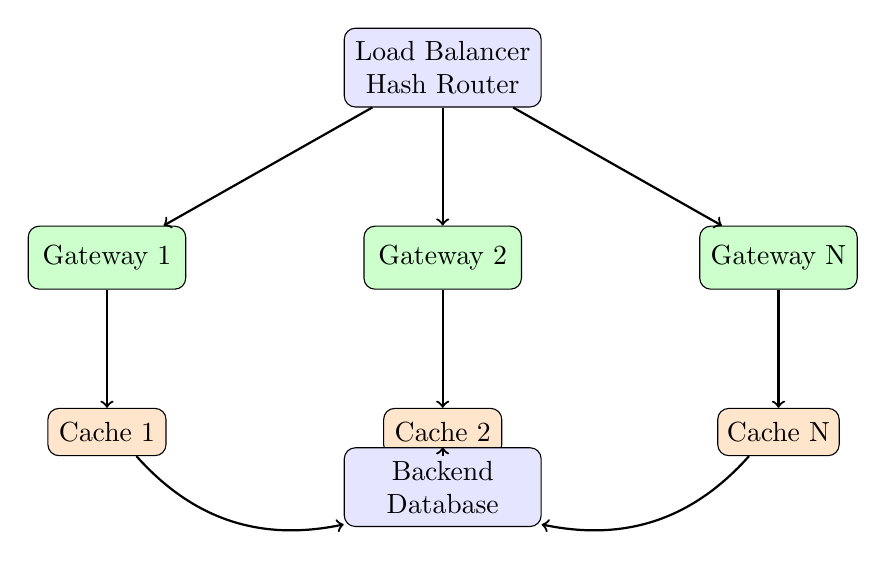
\begin{tikzpicture}[
    box/.style={draw, rectangle, rounded corners, fill=blue!10,
                minimum width=2.5cm, minimum height=1cm, align=center},
    gateway/.style={draw, rectangle, rounded corners, fill=green!20,
                    minimum width=2cm, minimum height=0.8cm},
    cache/.style={draw, rectangle, rounded corners, fill=orange!20,
                  minimum width=1.5cm, minimum height=0.6cm},
    arrow/.style={->, thick},
    node distance=1.5cm and 2cm
]
\node[box] (lb) {Load Balancer \\ Hash Router};
\node[gateway, below left=of lb] (gw1) {Gateway 1};
\node[gateway, below=of lb] (gw2) {Gateway 2};
\node[gateway, below right=of lb] (gw3) {Gateway N};
\node[cache, below=of gw1] (cache1) {Cache 1};
\node[cache, below=of gw2] (cache2) {Cache 2};
\node[cache, below=of gw3] (cache3) {Cache N};
\node[box, below=2cm of gw2] (backend) {Backend \\ Database};

\draw[arrow] (lb) -- (gw1);
\draw[arrow] (lb) -- (gw2);
\draw[arrow] (lb) -- (gw3);
\draw[arrow] (gw1) -- (cache1);
\draw[arrow] (gw2) -- (cache2);
\draw[arrow] (gw3) -- (cache3);
\draw[arrow] (cache1) to[bend right=30] (backend);
\draw[arrow] (cache2) -- (backend);
\draw[arrow] (cache3) to[bend left=30] (backend);
\end{tikzpicture}
\caption{Distributed deployment with hash routing.  Each fixture ID
         always reaches the same gateway, maximizing local hit ratio.}
\label{fig:hash-routing}
\end{figure}

\subsection{Circuit Breakers}

Circuit breakers wrap the backend calls made by the miss solver.  When
the backend is failing, the circuit breaker opens and the solver returns
\texttt{nullptr} (negative caching), preventing cascade failures.  This
is external to the cache library.

\begin{figure}[htbp]
\centering
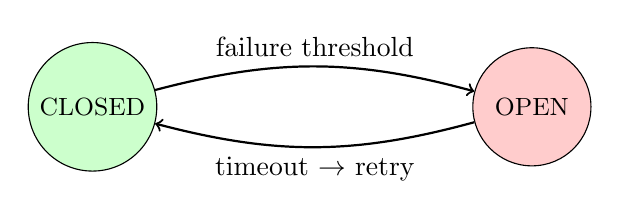
\begin{tikzpicture}[
    state/.style={circle, draw, minimum size=1.5cm, font=\small,
                  align=center},
    arrow/.style={->, thick},
    node distance=4cm
]
\node[state, fill=green!20] (closed) {CLOSED};
\node[state, fill=red!20, right=of closed] (open) {OPEN};

\draw[arrow] (closed) to[bend left=15] node[above] {failure threshold} (open);
\draw[arrow] (open) to[bend left=15] node[below] {timeout $\to$ retry} (closed);
\end{tikzpicture}
\caption{Simplified circuit breaker states.  When open, the solver
         returns \texttt{nullptr} immediately (negative caching protects
         the backend).}
\label{fig:circuit-breaker}
\end{figure}

\subsection{Failover}

When a gateway fails, Kubernetes redistributes traffic to surviving
instances, causing massive cache misses (cold cache problem).

\begin{figure}[htbp]
\centering
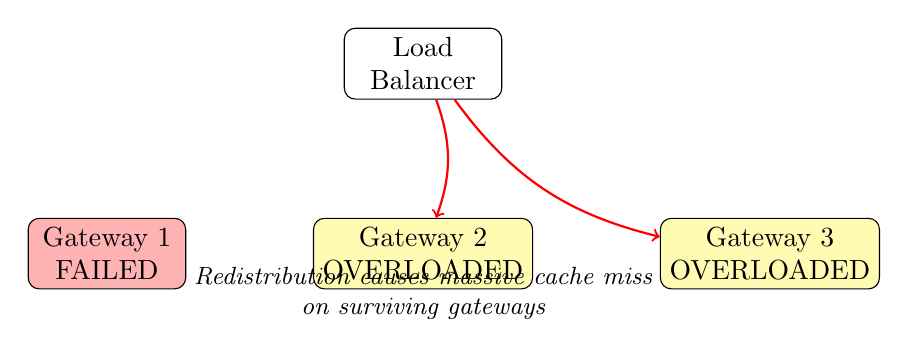
\begin{tikzpicture}[
    box/.style={draw, rectangle, rounded corners, minimum width=2cm,
                minimum height=0.8cm, align=center},
    failed/.style={draw, rectangle, rounded corners, fill=red!30,
                   minimum width=2cm, minimum height=0.8cm, align=center},
    overloaded/.style={draw, rectangle, rounded corners, fill=yellow!30,
                       minimum width=2cm, minimum height=0.8cm,
                       align=center},
    arrow/.style={->, thick},
    redarrow/.style={->, thick, red},
    node distance=1.5cm and 2cm
]
\node[box] (lb1) {Load \\ Balancer};
\node[failed, below left=of lb1] (gw1) {Gateway 1 \\ FAILED};
\node[overloaded, below=of lb1] (gw2) {Gateway 2 \\ OVERLOADED};
\node[overloaded, below right=of lb1] (gw3) {Gateway 3 \\ OVERLOADED};

\draw[redarrow] (lb1) to[bend left=20] (gw2);
\draw[redarrow] (lb1) to[bend right=20] (gw3);

\node[below=2cm of lb1, align=center, font=\small\itshape]
  {Redistribution causes massive cache miss\\on surviving gateways};
\end{tikzpicture}
\caption{Failover scenario.  Traffic redistribution after a gateway
         failure causes cold-cache storms on the remaining instances.
         A hot/standby model is under evaluation.}
\label{fig:failover}
\end{figure}

% ===================================================================
\section{Promela Model Overview}

The Promela model (\texttt{formal/cache\_model.pml}) provides exhaustive
verification of the concurrency protocol:

\begin{itemize}
\item \textbf{Capacity}: 2 slots, 3 keys, 6 request threads + 4
      background processes.
\item \textbf{State vector}: 152 bytes.
\item \textbf{State space}: $\sim$3.5 million states explored
      exhaustively.
\item \textbf{Verification time}: $\sim$4 seconds on modern hardware.
\end{itemize}

\subsection{What is Modeled}

\begin{itemize}
\item Refcount semantics (\texttt{slot\_rc[]} $\leftrightarrow$
      \texttt{CacheEntry::\_refcount} + EntryGuard RAII)
\item TTL aging (\texttt{slot\_age[]} with threshold $\leftrightarrow$
      sliding-window TTL)
\item All public API methods
\item LRU eviction with refcount guard (\texttt{rc $\leq$ 1})
\item Three-phase locking protocol
\item CV wait semantics (non-owners block on Computing entries)
\end{itemize}

\subsection{What is Abstracted}

\begin{itemize}
\item Exact wall-clock timing (replaced by discrete aging steps)
\item Hash table collision resolution details
\item Value content (only state transitions matter)
\item Deployment-level concerns (circuit breakers, routing)
\end{itemize}

\end{document}
